\chapter{Design and Architecture}
\section{Design}
The design of software application needs a well defined problem, when a new improved design of a user interface is needed. Main focus lays in easy navigation, responsive interface and intuitive access to the most needed parts of the system. \todo{rewrite introduciont to chapter}.

\subsection{The focus}
The focus of new design lays in improving the user experience. This application is integrateing GitHub for safe login system, access to git repositories through authentication, and gives the user easy controll over the repositories relevant to specific courses. The system is designed is such a way so that both students and teachers have intuitive access to the parts of the system that they use most frequently. There exists student section and teacher section, these are called "modes"\worry{insert something about admin mode?}, having Autograder in teacher mode, one can easily create a new course and rename it, GitHub integration \ref{gihubintegration} takes care of creating and managing the repositories needed in that course, initial setup of a course is done through a course setup page. The management of students that have joined the course, involves actions like creating group assignments, expelling students and approving new studends who joined the course, these can be done in the course management page. Most used functionality, by both teachers and teaching assistants is course lab overview. This lets a teacher quickly skim through all the students and look if anyone hasn't delivered their assignment yet, or see the score of each assignment, from there, it is also possible to approve or reject any given lab assignment. Another function is to be able to easily controll group assignments, and assign students to specific groups. In the group management page, there exists a user friendly interface for creating new groups and adding available students to any given group, users can be notyfied about which group they have been assigned to, similarly, students can easily create groups that need to be approved by the teachers. Students will utilize Autograder manilny for checking if their assignment has been approved. The default page for student mode is lab overview, there one can see the current assignment and its progress, the default course is the one choosen on last session when the user was logged in, it is also worth mentioning that usually one student wont be using Autograder in more than one course, but the system is designed for easy switch between different courses. Another userbase for Autograder are teaching assistants, they are both students and teachers in other courses, this is where Autograder modes come in handy, while working as a TA, user can switch to teacher mode and has access to the teaches functionality in the courses he teaches, similarly switching to student mode gives quick access to relevat functions in that mode.
\subsection{Planning of software solutions}
To achieve the goal of better, quicker and more responsive interface, the front-end application is written in JavaScript. By using new emerging open source technologies and libraries like React.js, it enabled quick and easy way to create a responsive user interface. \worry{explain it differently, depending on how much was written in background} In Model View Controller (more about it in section \ref{sec:mvc}) React would stand for View, that is what user sees, and interacts with. What is missing is something to controll the user interface and the datastructures that it displays. This is achieved by structuring the application with one of many popular software architectures that are practiced nowadays. Slightly altered way of doing things than previous MVC implementations was introduced with Flux architecture. The way to write code by flux  pattern is to isolate every UI component and send every updated piece of thata through a central hub that will dispach it further, and other components can be set up to listen to those specific changes they are interested in, more about Flux in section \ref{sec:flux}.
\\
\todo{introduce websockets here 250+ words}
\subsection{User stories}
User stories are a way to describe what application does, and what it is supposed to do in easy to read short descriptions. The focus here is to give a good fundament of what the applications is being developed for. Since there is a lot of functionality to be implementet, with the help of user stories is is possible to concentrate on one functionality described by that user story at a time. One example of a user storie would be \emph{"As a teacher I want to be able to easily create groups for assignments, so that i don't have to approve student created groups."} fig: \ref{fig:groupmanagement}, \worry{choose better user story maby?} this describes vaguely what a certain user would like to do with the application, but also can be created as a starting point for improvement to existing solution. It is also possible, by looking at this user story, to create a set of tasks that will guide through the steps of implementation. If there are parts of the system that need to be thought out again, or new solutions are needed to be in place before this functionality can be implemented, it is considered a part of the user story task. \worry{ With each new user story, the complexity of the application grows, and user interface should be theoretically improving on each cycle due to the way in which new functionality is implemented, since the flow of the application is being thought out and some initial design flaws might be discovered, things need to be either redesigned or a new solution found before this new functionality can be implemented. }\todo{More}

\subsection{Wireframes}
Creating wireframes is a crucial part of user interface design. The point of wireframes is to have something that is easier to change than the code to be developed. Before coming to the programming phase, one can iterate over a lot more design propositions, and is able to change things up easily during this initial or planning phase. Wireframes are foundation of the application being developed, they are not supposed to show the creative design, but rather reflect on the technological and use-related aspects of the application. Before the development of new user story takes action, sketches and drawings of user interface are being produced. This is done to eliminate flaws in the interface design before they are implemented, a couple of iterations of drawing are done and evalueted from the users perspective. When this initial phase is done, more sophisticated drawings or wireframes are being created. These more detailed drawings with descriptions of areas of the interface, describe what certain elements of this user interface do. Serving as a blue print for further developing of the interface.
\begin{figure}[h]
  {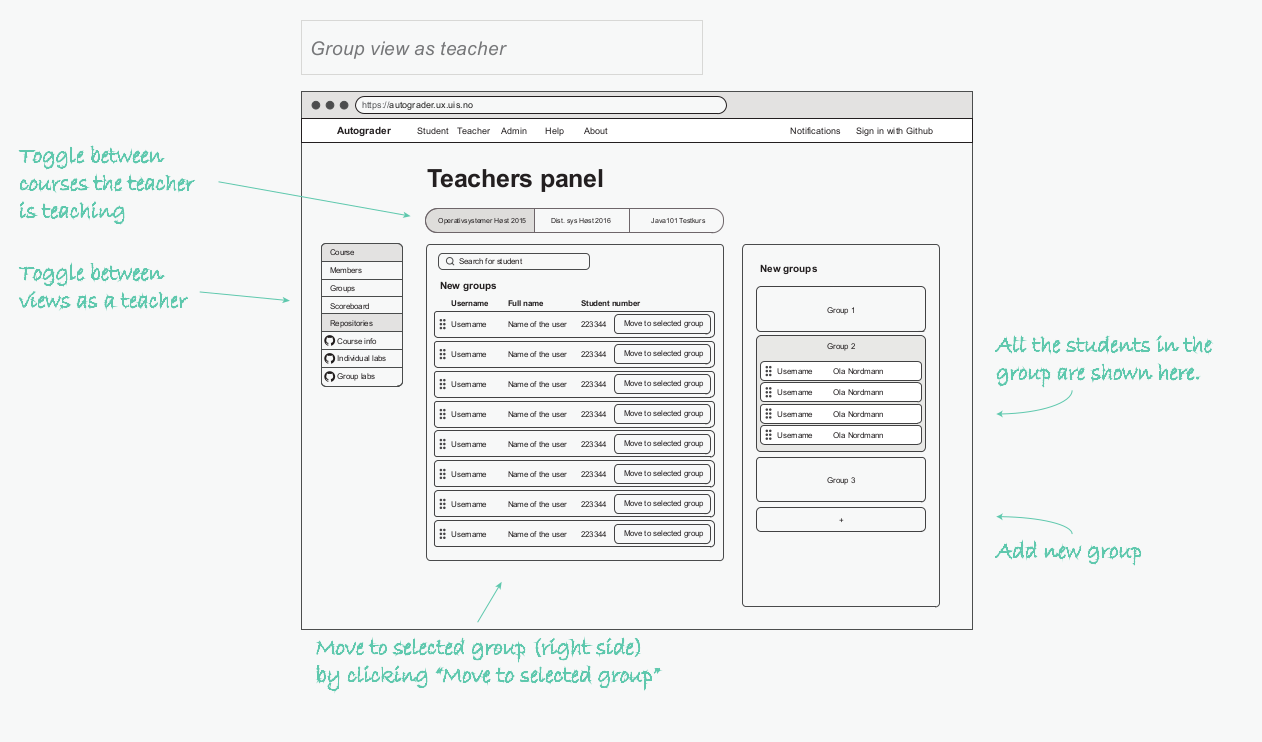
\includegraphics[width=1\linewidth]{groupmanagement}}
  \caption{Wireframes for Group management page}
  \label{fig:groupmanagement}
\end{figure}
\\Wireframe figure above was created as a result of a user story, next step is to create reflection of that wireframe in code, 


\section{Development process}
\worry{not sure about this section, is it usefoul for the reader?}\\
What enables us to finish the design as it was planned is good workflow, this is there are a couple of ways to go about it, they improve the effectivity and productivity of the process of developing new software solution.
\subsection{Kanban / Scrum}
\todo{explain short kanban and scrum}

\section{Architecture}
Architecture of the Autograder system describes the high level structures developed while working on the application. Choice of software architecture, software models on both front and back-end are things that are crucial aspects of creating good application.
\subsection{Software architecture}
Autograder is an application for teachers and students, the new version is going to be running on local university network and is going to be accessible from anywhere on the internet, that means there is no restrictions as to what network you are trying to access it from. Primary use for teachers is creating courses in the Autograder system that are associated with the courses at the university, each course has a GitHub repository associated with it, and configured to the needs of that course. This means that an implementation of GitHub integration needs to be created, this is mainly the focus of back-end part of the software, still the front-end, or web client, needs to be designed in such a way to enable the use such integration. The client is not supposed to serve as an alternative view of GitHub repositories, GitHub is mainly used as a place to easily store source code, and its authentication system. The client needs to be able to display courses that a student is enrolled into, assignments that the teacher has published to that course, that also involves group assignments.
\\Although the data is stored in the databse, manipulation of that data is done on the client side, and then sent further to the back-end for interpretation and updating the storage. Similarly it is also possible to update the client from the back-end, either directly or through the actions of another client. The user interface updates in real time, as an example, lets take a teacher that is assigning students to group assignmets, teacher is using an interactive interface to manipulate the users into selected groups, the student is simultaneusly notfied in real time when he gets assigned to a new group withouth the need of refreshing the page \worry{better example here}. Teachers can be notified when a new student has enrolled to course, or one of the students has exceeded his slip-days for an assignment. Real time updates are possible due to the connection protocol used in the application. When a client connects to the autogader server, client application requests for a protocol upgrade, from then on all data transfer is done through \emph{websocket prodocol}\cite{websocket}. This enables the server to push its updates to all clients, without being explicetly asked about it by them.
\\The reasoning behind real-time update system was that notifications and responsiveness of user interface was one of the primary reasons for developing this application. Although one could argue that orther methos of updating the UI and notifications would be sufficient, like polling or long-polling, that is frequent client requests for update from the server, websocket protocol has no obvoius disatvantages to the presented solution, and at the same time opens possibilities for further upgrades of the system, like chat functionality, which could be utilized for questions related to assignments.
\subsection{MVP or Model View Controller}\label{sec:mvc}

\subsection{Flux}\label{sec:flux}

\subsection{Other}

\subsection{Backend}
Backend solution is not the main focus of this application. Nonetheless a working temporary server needed to be put together, as well as database to store mock data and to test the logical functionallity of the system on the fron-end and the way the data is being communicated between the two ends.
\subsubsection{Server}
The server is written in Go \emph{Golang}, for this purpose there was no real  preference as to what language to use, but assumptions were made that the final server will also be written in go, therefore it was a clear choice. The Autograder server is going to be handling about 100 clinets at once, \worry{not event that many, rewrite later} this is not a big number, but the possibility is that it will grow in the future. The problem that arose during the development was the way in which the server should handle the clients. As discuissed earlier, the client requests for protocol upgrade to websocket protocol, this means that only the initial handshake is done through http, this removes any need for further http related requests. Before the websocked were implementet on the client side, the plan was to use a library called gorilla/mux, a multiplexer to easily handle different url, and assign handle funcitons to them. When websocket on the clientside where implemented, realization occured that the multiplexer for http requests will not be used at all, but on the other hand the way to handle the websocket payloads will have to be implemented. \worry{There exists a simple switch statement that handles the payloads through websocket, this will have to be worked on a bit more, as it is now we will not discusse it further at this point in time}
\subsubsection{Database}
Database is another part not central to the application, but just like the server, it was neccessary to implement it so that it becomes easier to see the whole flow of the program.
\\SQL database was designed first in a dia \emph{(drawing program)} \worry{and not changed since}
\subsection{Frontend}
\todo{single threaded approche}
\subsubsection{Angular}
\todo{discuisse other methods than react, needs more research}
\subsection{React}
\todo{Would we use react for this purpose again?}
